\documentclass[tikz,border=10pt]{standalone}
\usepackage[T1]{fontenc}
\usepackage{tikz}
\usetikzlibrary{positioning}
\begin{document}
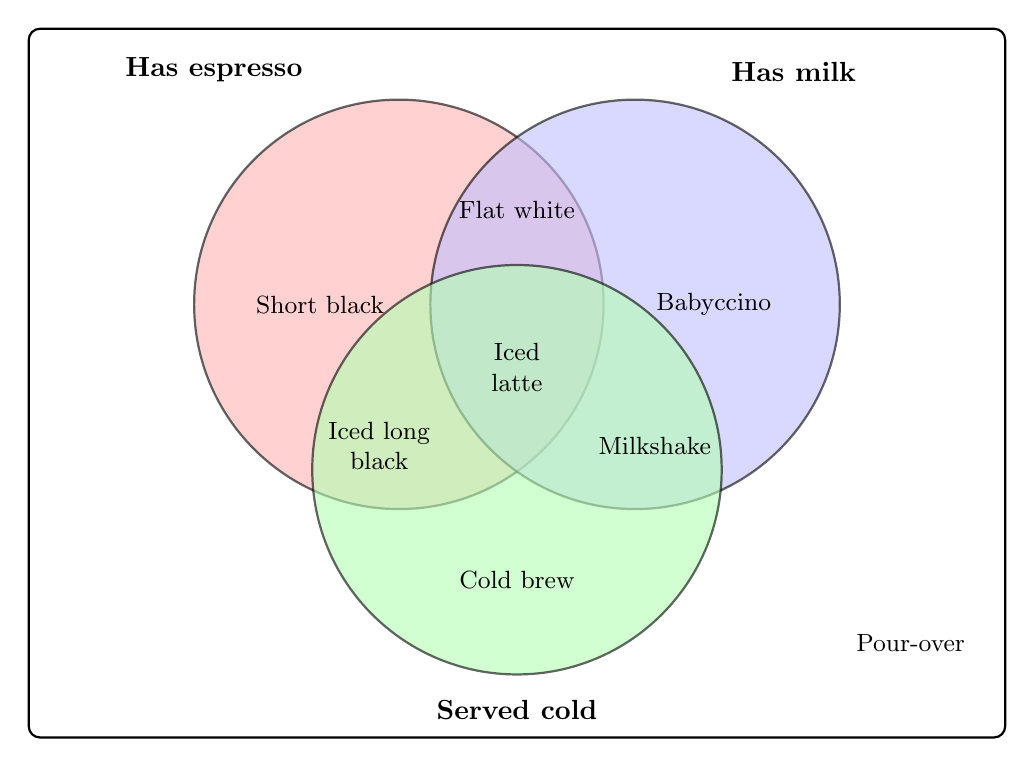
\begin{tikzpicture}[
  every node/.style={font=\small, align=center},
  setlabel/.style={font=\bfseries\normalsize},
]
  % universal set
  \draw[rounded corners=4pt, thick] (-6.2,-4.6) rectangle (6.2,4.4);

  % three circles
  \coordinate (E) at (-1.5,0.9);
  \coordinate (M) at (1.5,0.9);
  \coordinate (C) at (0,-1.2);
  \draw[thick, fill=red!30,   opacity=0.6] (E) circle (2.6);
  \draw[thick, fill=blue!25,  opacity=0.6] (M) circle (2.6);
  \draw[thick, fill=green!30, opacity=0.6] (C) circle (2.6);

  % set labels
  \node[setlabel, anchor=south east] at (-2.6,3.6) {Has espresso};
  \node[setlabel, anchor=south west] at (2.6,3.6) {Has milk};
  \node[setlabel, anchor=north] at (0,-4.0) {Served cold};

  % regions
  \node at (-2.5,0.9) {Short black};
  \node at (2.5,0.9) {Babyccino};
  \node at (0,-2.6) {Cold brew};
  \node at (0,2.1) {Flat white};
  \node at (-1.75,-0.9) {Iced long\\black};
  \node at (1.75,-0.9) {Milkshake};
  \node at (0,0.1) {Iced\\latte};
  \node at (5.0,-3.4) {Pour-over};
\end{tikzpicture}
\end{document}
